\let\negmedspace\undefined
\let\negthickspace\undefined
\documentclass[journal,12pt,onecolumn]{IEEEtran}
\usepackage{cite}
\usepackage{amsmath,amssymb,amsfonts,amsthm}
\usepackage{algorithmic}
\usepackage{graphicx}
\usepackage{textcomp}
\usepackage{xcolor}
\usepackage{txfonts}
\usepackage{listings}
\usepackage{enumitem}
\usepackage{mathtools}
\usepackage{gensymb}
\usepackage{comment}
\usepackage[breaklinks=true]{hyperref}
\usepackage{tkz-euclide} 
\usepackage{gvv}                                        
%\def\inputGnumericTable{}                                 
\usepackage[latin1]{inputenc}     
\usepackage{xparse}
\usepackage{color}                                            
\usepackage{array}                                            
\usepackage{longtable}                                       
\usepackage{calc}                                             
\usepackage{multirow}
\usepackage{multicol}
\usepackage{hhline}                                           
\usepackage{ifthen}                                           
\usepackage{lscape}
\usepackage{tabularx}
\usepackage{float}
\newtheorem{theorem}{Theorem}[section]
\newtheorem{problem}{Problem}
\newtheorem{proposition}{Proposition}[section]
\newtheorem{lemma}{Lemma}[section]
\newtheorem{corollary}[theorem]{Corollary}
\newtheorem{example}{Example}[section]
\newtheorem{definition}[problem]{Definition}
\newcommand{\BEQA}{\begin{eqnarray}}
\newcommand{\EEQA}{\end{eqnarray}}
\newcommand{\define}{\stackrel{\triangle}{=}}
\theoremstyle{remark}
\newtheorem{rem}{Remark}
% Marks the beginning of the document
\begin{document}
\title{PI : PRODUCTION AND INDUSTRIAL ENGINEERING}
\author{AI25BTECH11034 - Sujal Chauhan}
\maketitle
\renewcommand{\thefigure}{\theenumi}
\renewcommand{\thetable}{\theenumi}
\textbf{\Large Genral Aptitude } \\
\vspace{1cm}
\textbf{\large Q.1 - Q.5 carry one mark each}
\begin{enumerate}
% Q.1
\item While I agree \underline{\hspace{2cm}} his proposal this time, I do not often agree  him.
\hfill{(GATE 2020)}
\begin{multicols}{4}
\begin{enumerate}
    \item to, with
    \item with, to
    \item with, with
    \item to, to
\end{enumerate}
\end{multicols}
\vspace{1cm}

% Q.2
\item The recent measures to improve the output would \underline{\hspace{2cm}}the level of production to our satisfaction.
\hfill{(GATE 2020)}
\begin{multicols}{4}
\begin{enumerate}
    \item increase
    \item decrease
    \item speed
    \item equalise
\end{enumerate}
\end{multicols}
\vspace{1cm}

% Q.3
\item Select the word that fits the analogy: \\
White : Whitening :: Light : \underline{\hspace{2cm}}  
\hfill{(GATE 2020)}
\begin{enumerate}
    \item Lightning
    \item Lightening
    \item Lighting
    \item Enlightening
\end{enumerate}
\vspace{1cm}

% Q.4
\item In one of the greatest innings ever seen in 142 years of Test history, Ben Stokes upped the tempo in a five-and-a-half hour long stay of 219 balls including 11 fours and 8 sixes that saw him finish on 135 not out as England squared the five-match series.

Based on their connotations in the given passage, which one of the following meanings DOES NOT match?
\hfill{(GATE 2020)}
\begin{multicols}{4}
\begin{enumerate}
    \item upped = increased
    \item squared = lost
    \item tempo = enthusiasm
    \item saw = resulted in
\end{enumerate}
\end{multicols}
\vspace{1cm}
\newpage
% Q.5
\item There are five levels (\{P, Q, R, S, T\}) in a linear supply chain before a product reaches customers, as shown in the figure.
\hfill{(GATE 2020)}

\begin{figure}[H]
    \centering
    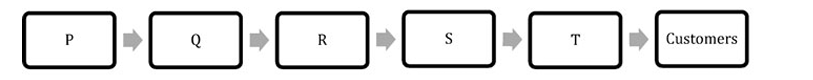
\includegraphics[width=0.65\linewidth]{GATE-PI-2020/5a.png} 
    \caption{}
    \label{q5a}
\end{figure}

At each of the five levels, the price of the product is increased by 25\%. If the product is produced at level P at the cost of Rs. 120 per unit, what is the price paid (in rupees) by the customers?
\begin{multicols}{4}
\begin{enumerate}
    \item 187.50
    \item 234.38
    \item 292.96
    \item 366.21
\end{enumerate}
\end{multicols}
\vspace{1cm}
\textbf{\large Q.6 - Q.10 carry two mark each}
% Q.6
\item Climate change and resilience deal with two aspects a reduction of sources of non-renewable energy resources and reducing vulnerability of climate change aspects. The terms amitigationa and adaptationa are used to refer to these aspects, respectively.

Which of the following assertions is best supported by the above information?
\hfill{(GATE 2020)}

\begin{enumerate}
    \item Mitigation deals with consequences of climate change.
    \item Adaptation deals with causes of climate change.
    \item Mitigation deals with actions taken to reduce the use of fossil fuels.
    \item Adaptation deals with actions taken to combat green-house gas emissions.
\end{enumerate}

\vspace{1cm}

% Q.7
\item Find the missing element in the following figure.
\hfill{(GATE 2020)}

\begin{figure}[H]
    \centering
    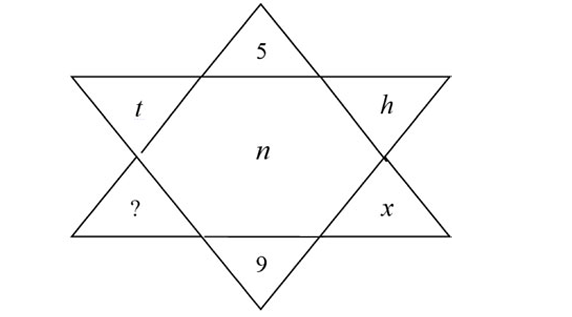
\includegraphics[width=0.35\linewidth]{GATE-PI-2020/7a.png} 
    \caption{}
    \label{q7a}
\end{figure}

\begin{multicols}{4}
\begin{enumerate}
    \item $4$
    \item $6$
    \item $7$
    \item $8$
\end{enumerate}
\end{multicols}
\vspace{1cm}

% Q.8
\item It was estimated that $52$ men can complete a strip in a newly constructed highway connecting cities $P$ and $Q$ in $10$ days. Due to an emergency, $12$ men were sent to another project. How many number of days, more than the original estimate, will be required to complete the strip?
\hfill{(GATE 2020)}
\begin{multicols}{4}
\begin{enumerate}
    \item $3$ days
    \item $5$ days
    \item $10$ days
    \item $13$ days
\end{enumerate}
\end{multicols}
\vspace{1cm}

% Q.9
\item An engineer measures THREE quantities X, Y and Z in an experiment. She finds that they follow a relationship that is represented in the figure below: (the product of X and Y linearly varies with Z)

\begin{figure}[H]
    \centering
   
    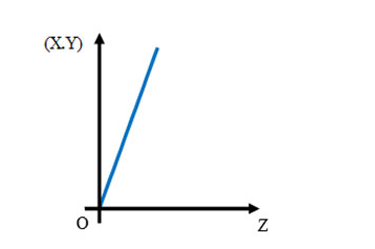
\includegraphics[width=0.35\linewidth]{GATE-PI-2020/9a.png}
    \caption{}
    \label{q9a}
\end{figure}

Then, which of the following statements is FALSE?
\begin{enumerate}
    \item For fixed $X$, $Z$ is proportional to $Y$
    \item For fixed $Y$, $Z$ is proportional to $X$
    \item For fixed $X$, $Y$ is proportional to $Z$
    \item $XYZ$ is constant
\end{enumerate}
\vspace{1cm}
% Q.10
\item The two pie-charts given below show the data of total students and only girls registered in different streams in a university. If the total number of students registered in the university is 5000, and the total number of the registered girls is 1500; then, the ratio of boys enrolled in Arts to the girls enrolled in Management is \underline{\hspace{1.5cm}}.
\hfill{(GATE 2020)}

\begin{figure}[H]
    \centering
    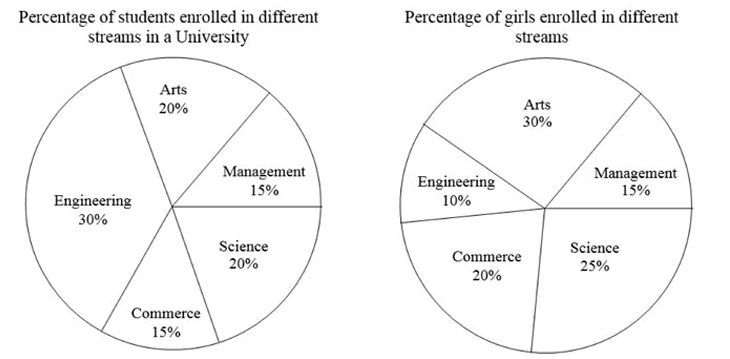
\includegraphics[width=0.43\linewidth]{GATE-PI-2020/10a.png} 
   
  
\end{figure}

\begin{multicols}{4}
\begin{enumerate}
    \item $2:1$
    \item $9:22$
    \item $11:9$
    \item $22:9$
\end{enumerate}
\end{multicols}
\vspace{1cm}
\end{enumerate}

\newpage
\textbf{PI:}
\textbf{\large Q.1 - Q.25 carry one mark each}
\begin{enumerate}
  
% Q.1
\item The divergence of the vector $\vec{v} = y z^2 \hat{i} + z x^2 \hat{j} + x^2 \hat{k}$ is 
\hfill{(GATE 2020)}
\begin{multicols}{4}
\begin{enumerate}
    \item $2x$
    \item $2y$
    \item $2z$
    \item $0$
\end{enumerate}
\end{multicols}
\vspace{1cm}

% Q.2
\item An integrating factor for the differential equation $\dfrac{dy}{dx} + my = e^{-mx}$ is  
\hfill{(GATE 2020)}
\begin{multicols}{4}
\begin{enumerate}
    \item $e^{m}$
    \item $e^{-m}$
    \item $e^{-mx}$
    \item $e^{mx}$
\end{enumerate}
\end{multicols}
\vspace{1cm}

% Q.3
\item For the complex numbers $z_1 = 2 + 3i$ and $z_2 = 4 - 5i$, the value of $(z_1 + z_2)^2$ is  
\hfill{(GATE 2020)}
\begin{multicols}{4}
\begin{enumerate}
    \item $32 - 24i$
    \item $-32 - 24i$
    \item $32 + 24i$
    \item $-32 + 24i$
\end{enumerate}
\end{multicols}
\vspace{1cm}

% Q.4
\item To solve $x^2 - 2 = 0$, the Newton-Raphson method has been employed. If the initial guess $x_0 = 1.0$, the next estimate of the root, $x_1$, will be  
\hfill{(GATE 2020)}
\begin{multicols}{4}
\begin{enumerate}
    \item $0.5$
    \item $1.0$
    \item $1.5$
    \item $2.0$
\end{enumerate}
\end{multicols}
\vspace{1cm}
% Q.5
\item If $x$ is a random variable with the expected value of $5$ and the variance of $1$, then the expected value of $x^2$ is
\hfill{(GATE 2020)}
\begin{multicols}{4}
\begin{enumerate}
    \item $24$
    \item $25$
    \item $26$
    \item $36$
\end{enumerate}
\end{multicols}
\vspace{1cm}

% Q.6
\item Group I lists phases of steel and Group II lists crystal structures in the table below.

\begin{center}
\begin{tabular}{|c|l|c|l|}
\hline
\textbf{Group I} & & \textbf{Group II} & \\
\hline
P. Ferrite & & 1. Hexagonal Close Packed (HCP) & \\
Q. Austenite & & 2. Body Centered Cubic (BCC) & \\
R. Martensite & & 3. Body Centered Tetragonal (BCT) & \\
             & & 4. Face Centered Cubic (FCC) & \\
\hline
\end{tabular}
\end{center}

Match the phase with the corresponding crystal structure.
\begin{multicols}{4}
\begin{enumerate}
    \item P-2, Q-4, R-3
    \item P-4, Q-2, R-3
    \item P-2, Q-4, R-1
    \item P-4, Q-2, R-1
\end{enumerate}
\end{multicols}
\vspace{1cm}
\newpage
% Q.7
\item The figure shows two bodies P and Q. The body Q is placed on the ground and the body P is placed on top of it. The weights of P and Q are $W_P$ and $W_Q$, respectively. The bodies are at rest and all the surfaces are assumed to be frictionless. $R$ represents reaction force, if any, between the bodies.

\begin{figure}[H]
    \centering
    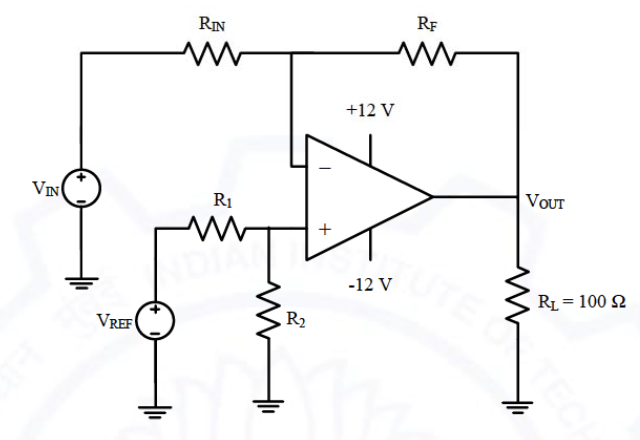
\includegraphics[width=0.25\linewidth]{GATE-PI-2020/7.png}
    \caption{}
    \label{7}
\end{figure}

The correct free body diagram of the body P is
\begin{enumerate}
    \item 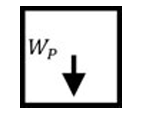
\includegraphics[height=2.2cm]{GATE-PI-2020/7aa.png} 
    \item 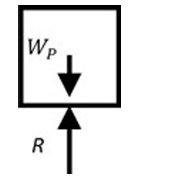
\includegraphics[height=2.2cm]{GATE-PI-2020/7b.png} 
    \item 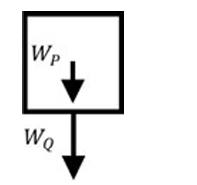
\includegraphics[height=2.2cm]{GATE-PI-2020/7c.png}
    \item 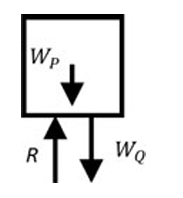
\includegraphics[height=2.2cm]{GATE-PI-2020/7d.png}
\end{enumerate}
\vspace{1cm}

% Q.8
\item The figure shows a mechanism with $3$ revolute pairs (between the links $1$ and $2$, $2$ and $3$, and $3$ and $4$) and a prismatic pair (between the links $1$ and $4$). Which one of the four links should be fixed to obtain the mechanism that forms the basis of the quick-return mechanism widely used in a shaper?
\begin{figure}[H]
    \centering
    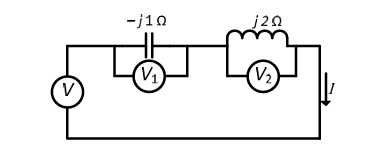
\includegraphics[width=0.5\linewidth]{GATE-PI-2020/8.png} 
    \caption{}
    \label{8}
\end{figure}
\begin{multicols}{4}
\begin{enumerate}
    \item Link 1
    \item Link 2
    \item Link 3
    \item Link 4
\end{enumerate}
\end{multicols}
\vspace{1cm}

% Q.9
\item The state of stress at a point in a body under plane stress condition is shown in the figure. The positive directions of $x$ and $y$ axes are also shown. The material of the body is homogeneous and isotropic, with modulus of elasticity $E$ and Poisson's ratio $\nu$. The longitudinal strain in the $x$direction is
\begin{figure}[H]
    \centering
    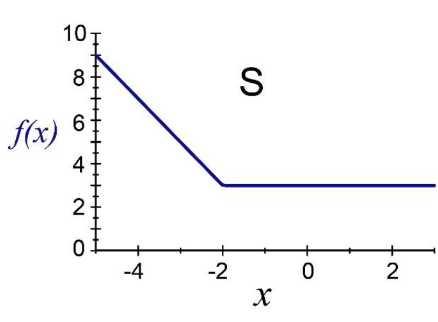
\includegraphics[width=0.27\linewidth]{GATE-PI-2020/9.png} % Replace with actual stress diagram filename
    \caption{}
    \label{fig:planestress}
\end{figure}
\begin{multicols}{4}
\begin{enumerate}
    \item $\frac{\sigma_x}{E} - \nu\frac{\sigma_y}{E}$
    \item $\frac{\sigma_x}{E} - \frac{\sigma_y}{\nu E}$
    \item $\frac{\sigma_x}{E} + \frac{\sigma_y}{E}$
    \item $\frac{\sigma_x}{E} + \nu\frac{\sigma_y}{E}$
\end{enumerate}
\end{multicols}
\vspace{1cm}

% Q.10
\item The figure shows two bodies connected through a riveted joint with one rivet. The diameter of the rivet is $d$ (in m). The joint transmits a load of $F$ (in N) whose line of action is perpendicular to and intersects the vertical axis of the rivet. Neglect any effect of bending of the rivet. If the allowable shear stress for the material of the rivet is $\tau$ N/m$^2$, the diameter of the rivet required to prevent failure in shear is
\begin{figure}[H]
    \centering
    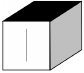
\includegraphics[width=0.4\linewidth]{GATE-PI-2020/10.png}
    \caption{}
    \label{fig:rivetjoint}
\end{figure}
\begin{multicols}{4}
\begin{enumerate}
    \item $ \sqrt{\dfrac{F}{\pi \tau}} $
    \item $ \sqrt{\dfrac{2F}{\pi \tau}} $
    \item $ \sqrt{\dfrac{4F}{\pi \tau}} $
    \item $ \sqrt{\dfrac{8F}{\pi \tau}} $
\end{enumerate}
\end{multicols}
\vspace{1cm}

% Q.11
\item Consider flow of an oil with Reynolds number $1500$ in a pipe of diameter $5$ cm. The kinematic viscosity of the oil, $\nu = 0.75$ cm$^2$/s. The value of average velocity in m/s is
\hfill{(GATE 2020)}
\begin{multicols}{4}
\begin{enumerate}
    \item $0.75$
    \item $1.50$
    \item $2.25$
    \item $4.50$
\end{enumerate}
\end{multicols}
\vspace{1cm}
\newpage
% Q.12
\item A Carnot heat engine receives $600$ kJ of heat per cycle from a source at $627^\circ$C and rejects heat to a sink at $27^\circ$C. The amount of heat rejected to the sink per cycle (rounded off to the nearest integer) in kJ is
\hfill{(GATE 2020)}
\begin{multicols}{4}
\begin{enumerate}
    \item $26$
    \item $200$
    \item $400$
    \item $574$
\end{enumerate}
\end{multicols}
\vspace{1cm}

% Q.13
\item The process used for producing long bars of fiber reinforced plastics (FRP) with uniform cross-section is
\hfill{(GATE 2020)}
\begin{multicols}{4}
\begin{enumerate}
    \item Extrusion
    \item Pultrusion
    \item Injection Molding
    \item Thermoforming
\end{enumerate}
\end{multicols}
\vspace{1cm}

% Q.14
\item The purpose of the ratchet in a micrometer is to
\hfill{(GATE 2020)}
\begin{enumerate}
    \item impart smooth movement to the spindle
    \item compensate for the wear of the screw thread
    \item prevent rotation of the spindle while reading the scale
    \item maintain sufficient and uniform measuring pressure
\end{enumerate}
\vspace{1cm}

% Q.15
\item End mill cutters are mounted on the spindle of a vertical milling machine using
\hfill{(GATE 2020)}
\begin{multicols}{4}
\begin{enumerate}
    \item vice
    \item collet
    \item face plate
    \item driver plate
\end{enumerate}
\end{multicols}
\vspace{1cm}

% Q.16
\item Self-sharpening tendency of a conventional grinding wheel depends upon
\hfill{(GATE 2020)}
\begin{multicols}{4}
\begin{enumerate}
    \item wheel structure
    \item wheel grade
    \item grit hardness
    \item grit size
\end{enumerate}
\end{multicols}
\vspace{1cm}

% Q.17
\item A non-traditional machining process which utilizes mechanical energy as the principal energy source for removing the material is
\hfill{(GATE 2020)}

\begin{enumerate}
    \item Electric discharge machining
    \item Laser beam machining
    \item Ultrasonic machining
    \item Plasma arc machining
\end{enumerate}

\vspace{1cm}

% Q.18
\item In manufacturing of self-lubricating bearings by powder metallurgy, an important secondary operation that is carried out after sintering is
\hfill{(GATE 2020)}

\begin{enumerate}
    \item Cold isostatic pressing
    \item Hot isostatic pressing
    \item Impregnation
    \item Infiltration
\end{enumerate}

\vspace{1cm}

% Q.19
\item Which of the following is a causal forecasting method?
\hfill{(GATE 2020)}

\begin{enumerate}
    \item Naive approach
    \item Moving average
    \item Exponential smoothing
    \item Linear regression
\end{enumerate}

\vspace{1cm}

% Q.20
\item An approach used in the product development which combines the efforts of design, manufacturing, and other functions to reduce the total time in introducing a new product in the market is
\hfill{(GATE 2020)}
\begin{multicols}{4}
\begin{enumerate}
    \item Concurrent engineering
    \item Lean manufacturing
    \item Value engineering
    \item Break-even analysis
\end{enumerate}
\end{multicols}
\vspace{1cm}

% Q.21
\item The Bellman's principle of optimality is related to
\hfill{(GATE 2020)}
\begin{multicols}{4}
\begin{enumerate}
    \item Linear programming problem
    \item Transportation problem
    \item Dynamic programming problem
    \item Assignment problem
\end{enumerate}
\end{multicols}
\vspace{1cm}

% Q.22
\item The process capability ratio $C_p$ is given by
\hfill{(GATE 2020)}
\begin{enumerate}
    \item 
    \[
    \frac{\text{Upper Specification Limit} - \text{Lower Specification Limit}}{6 \times \text{Process Standard Deviation}}
    \]
    \item 
    \[
    \frac{\text{Upper Control Limit} - \text{Lower Control Limit}}{6 \times \text{Process Standard Deviation}}
    \]
    \item 
    \[
    \frac{6 \times \text{Process Standard Deviation}}{\text{Upper Specification Limit} - \text{Lower Specification Limit}}
    \]
    \item 
    \[
    \frac{6 \times \text{Process Standard Deviation}}{\text{Upper Control Limit} - \text{Lower Control Limit}}
    \]
\end{enumerate}
\vspace{1cm}

% Q.23
\item In a uniaxial tensile test on a specimen of a ductile material, the ultimate tensile strength is found to be $400$ MPa and the elongation up to the maximum load is $25\%$. The true stress at the maximum load in MPa is \underline{\hspace{2cm}}.
\vspace{1cm}

% Q.24
\item Suppose the control system of a fighter jet consists of three unrelated components in series, and it is desired to have $98\%$ reliability of the system. If the reliability level of all the components is the same, then the reliability of each component (rounded off to three decimal places) is \underline{\hspace{2cm}}.
\vspace{1cm}

% Q.25
\item The product structure tree in the figure below shows the components needed to assemble one unit of product P.

\begin{figure}[H]
    \centering
    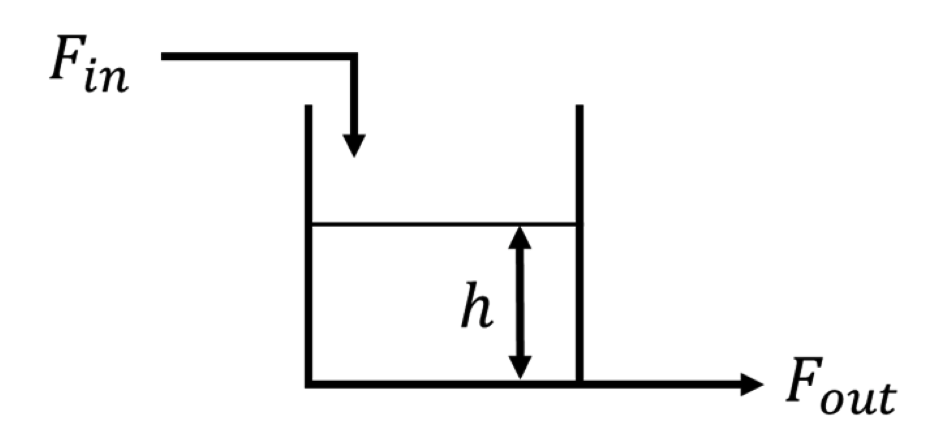
\includegraphics[width=0.6\linewidth]{GATE-PI-2020/25.png} 
    \caption{}
    \label{25}
\end{figure}

The number of units of component D needed to assemble 10 units of product P is \underline{\hspace{2cm}}.
\vspace{1cm}

\textbf{\large Q.26 - Q.55 carry two mark each}\\
\vspace{1cm}
% Q.26
\item General solution of $\displaystyle x^2 \frac{d^2y}{dx^2} + x \frac{dy}{dx} - y = 0$ is
\begin{enumerate}
    \item $y = \dfrac{C_1}{x} + \dfrac{C_2}{x^3}$
    \item $y = C_1 x^2 + \dfrac{C_2}{x^2}$
    \item $y = C_1 x + \dfrac{C_2}{x}$
    \item $y = C_1 x + C_2 x^3$
\end{enumerate}
\vspace{1cm}

% Q.27
\item For the matrix $\myvec{ 1 & 5 \\ 3 & 3 }$, the eigenvectors are
\begin{multicols}{2}
\begin{enumerate}
    \item $\myvec{-1 \\ 1}$ and $\myvec{3 \\ -3}$
    \item $\myvec{1 \\ 1}$ and $\myvec{-5/3 \\ 1}$
    \item $\myvec{1 \\ 3}$ and $\myvec{5/3 \\ 1}$
    \item $\myvec{-1 \\ 1}$ and $\myvec{5/3 \\ 1}$
\end{enumerate}
\end{multicols}
\vspace{1cm}

\newpage
% Q.28
\item A truss with two bars PR and QR, making angles $\alpha$ and $\beta$, respectively, with the vertical, is shown in the figure below. The connections at P, Q and R are hinged connections. The truss supports a body of weight $W$ (in N) at R as shown. The tension in the bar QR (in N) is
\begin{figure}[H]
    \centering
    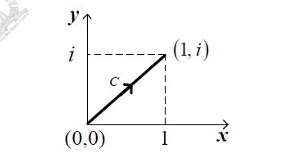
\includegraphics[width=0.35\linewidth]{GATE-PI-2020/28.png} 
    \caption{}
    \label{28}
\end{figure}
\begin{enumerate}
    \item $\dfrac{W \sin{\beta}}{\cos{(\alpha + \beta)}}$
    \item $\dfrac{W \cos{\beta}}{\sin{(\alpha + \beta)}}$
    \item $\dfrac{W \cos{\alpha}}{\cos{(\alpha + \beta)}}$
    \item $\dfrac{W \sin{\alpha}}{\sin{(\alpha + \beta)}}$
\end{enumerate}
\vspace{1cm}

% Q.29
\item The figure shows a beam of length $L$ (in m) with a uniformly distributed transverse load of $W$ (in N/m) acting over it. The width and depth of the beam cross section are $b$ (in m) and $t$ (in m), respectively. The magnitude of the maximum bending stress in the beam in N/m$^2$ is
\begin{figure}[H]
    \centering
    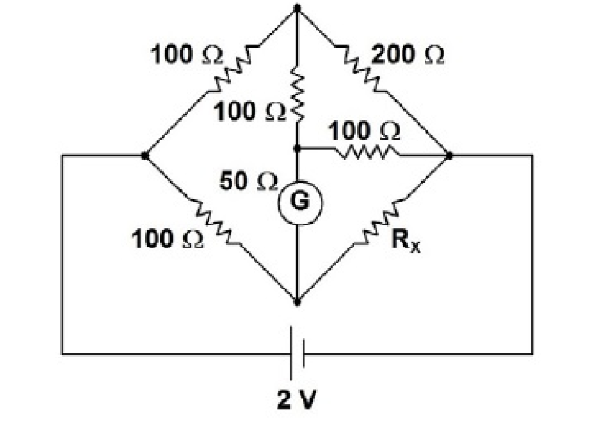
\includegraphics[width=0.5\linewidth]{GATE-PI-2020/29.png} 
    \caption{}
    \label{29}
\end{figure}
\begin{enumerate}
    \item $\dfrac{3 W L^2}{4 b t^2}$
    \item $\dfrac{4 W L^2}{3 b t^2}$
    \item $\dfrac{2 W L^2}{3 b t^2}$
    \item $\dfrac{3 W L^2}{2 b t^2}$
\end{enumerate}
\vspace{1cm}

% Q.30
\item The vertices of rectangle $PQRS$ are as follows in a 2-D CAD system.\\
$P(-4,-2);~Q(-2,-3);~R(-3,-5);~S(-5,-4)$.\\
The coordinates of the corresponding new vertices, $P', Q', R', S'$ after translation of the rectangle along x-axis in the positive direction by 6 units and along y-axis in the positive direction by 3 units are
\begin{multicols}{2}
\begin{enumerate}
    \item $P'(-10,-5);~Q'(-8,-6);~R'(-9,-8);~S'(-11,-7)$
    \item $P'(2,1);~Q'(4,0);~R'(3,-2);~S'(1,-1)$
    \item $P'(2,-5);~Q'(4,-6);~R'(3,-8);~S'(1,-7)$
    \item $P'(-10,1);~Q'(-8,0);~R'(-9,-2);~S'(-11,-1)$
\end{enumerate}
\end{multicols}
\vspace{1cm}

% Q.31
\item The statement that best describes the function of a GO gauge in the context of Taylor's principle of gauging is
\begin{enumerate}
    \item GO gauge checks the Maximum Material Condition and is designed to check as many dimensions as possible
    \item GO gauge checks the Least Material Condition and is designed to check as many dimensions as possible
    \item GO gauge checks the Maximum Material Condition and is designed to check only one dimension
    \item GO gauge checks the Least Material Condition and is designed to check only one dimension
\end{enumerate}
\vspace{1cm}

% Q.32
\item The figure shows revenue generated over different product life cycle stages marked as P, Q, R, and S. Group I lists these product life cycle stages. Group II lists typical efforts leading to revenue maximization during a stage.

\begin{figure}[H]
    \centering
    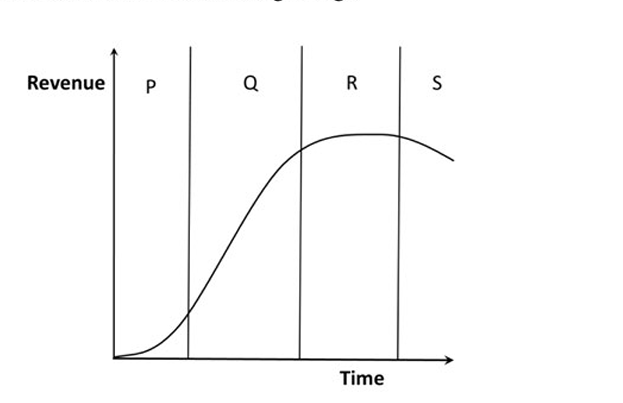
\includegraphics[width=0.5\linewidth]{GATE-PI-2020/32.png}
    \caption{}
    \label{32}
\end{figure}

\begin{tabular}{ll}
\textbf{Group I}     & \textbf{Group II} \\
P. Introduction      & 1. Efforts to enhance the production capacity \\
Q. Growth            & 2. Efforts to rejuvenate the product \\
R. Maturity          & 3. Efforts to maximize the product performance \\
S. Decline           & 4. Efforts to explore other markets \\
\end{tabular}

Match the stage with the efforts.
\begin{enumerate}
    \item P-3; Q-4; R-2; S-1
    \item P-1; Q-4; R-2; S-3
    \item P-1; Q-3; R-4; S-2
    \item P-3; Q-1; R-2; S-4
\end{enumerate}
\vspace{1cm}

% Q.33
\item A company manufactures products P and Q in quantities $x_1$ and $x_2$, respectively, using two resources. The following Linear Programming Problem (LPP) is formulated to maximize the profit $Z$.\\
Maximize $Z = 3x_1 + 2x_2$\\
subject to\\
$x_1 + 2x_2 \leq 2$ \quad (for Resource 1)\\
$2x_1 + x_2 \leq 2$ \quad (for Resource 2)\\
and $x_1, x_2 \geq 0$.\\
The shadow price for Resource 2 is
\begin{multicols}{4}
\begin{enumerate}
    \item $0$
    \item $\dfrac{2}{3}$
    \item $1$
    \item $\dfrac{4}{3}$
\end{enumerate}
\end{multicols}
\vspace{1cm}

% Q.34
\item A rectifying inspection is performed on a lot of size $N=1000$ using a Single-Sampling Plan with the sample size $n=60$ and the acceptance number $c=1$. If the Acceptable Quality Level is 1.0\%, the producer's risk associated with the sampling plan (rounded off to the nearest integer) in \% is \underline{\hspace{2cm}}.
\vspace{1cm}

% Q.35
\item For $y = -x^2 + 9x - 2$, the value of $\int_1^5 y dx$ using Simpson's $\frac{1}{3}$ rule with two intervals (rounded off to two decimal places) is \underline{\hspace{2cm}}.
\vspace{1cm}

% Q.36
\item If the probability density function of a random variable $x$ is given by
\[
f(x) = 
\begin{cases}
\dfrac{k x^2}{2}, & -1 \leq x \leq 1 \\
0, & \text{elsewhere}
\end{cases}
\]
the value of $k$ is \underline{\hspace{2cm}}.
\vspace{1cm}

% Q.37
\item A solid shaft has to transmit $50$ kW of power at a speed of $1910$ RPM. Ignore any possible bending of the shaft. The maximum allowable shear stress for the material of the shaft is $80$ MPa. The minimum diameter of the shaft required to prevent failure due to shear (rounded off to one decimal place) in cm is \underline{\hspace{2cm}}.
\vspace{1cm}

% Q.38
\item A flywheel is to be used in an IC engine to limit fluctuation of angular speed. The average of the maximum and the minimum angular speed is $500$ RPM, and the maximum fluctuation of energy is $10,000$ N-m. Neglecting rotary inertia of any other components, the moment of inertia of the flywheel about its axis of rotation required to limit the maximum fluctuation of speed to 30 RPM (rounded off to one decimal place) in kg-m$^2$ is \underline{\hspace{2cm}}.
\vspace{1cm}
\newpage
% Q.39
\item A tank of large cross-sectional area contains water up to a height of 5 m as shown in the figure.
The top water surface is under a pressure of $p_1 = 0.2$~MPa. A small, smooth, and round tap at the bottom of the tank is opened to the atmosphere ($p_2 = 0.1$~MPa).

\begin{figure}[H]
    \centering
    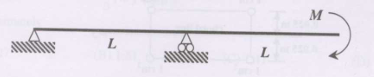
\includegraphics[width=0.5\linewidth]{GATE-PI-2020/39.png} 
    \caption{}
    \label{39}
\end{figure}

Use the acceleration due to gravity, $g = 9.81~\text{m}/\text{s}^2$ and the density of water, $\rho = 1000~\text{kg}/\text{m}^3$. The velocity with which the water will exit from the tap under the conditions shown in the figure (rounded off to one decimal place) in m/s is \underline{\hspace{2cm}}.
\vspace{1cm}

% Q.40
\item A steel ball of 12 mm diameter is heated to 1225~K. It is then slowly cooled in air to a temperature of 475~K. During the cooling process, the ambient temperature is 325~K and the heat transfer coefficient is 30~W/m$^2$-K. Assume, the density of steel is 7800~kg/m$^3$ and the specific heat is 600~J/kg-K. Using the lumped capacitance method of analysis, the calculated time for the required cooling (rounded off to one decimal place) in seconds is \underline{\hspace{2cm}}.
\vspace{1cm}

% Q.41
\item A mass of 3~kg of Argon gas at 3~bar, 27$^\circ$C is contained in a rigid, insulated vessel. Paddle wheel work is done on the gas for 30~minutes at the rate of 0.015~kW. Specific heat at constant volume, $C_v$, for Argon is 0.3122~kJ/kg-K. The final temperature of the gas (rounded off to one decimal place) in kelvin is \underline{\hspace{2cm}}.
\vspace{1cm}
\newpage
% Q.42
\item The figure shows drawing of a part with dimensions and tolerances, both in mm. The permissible tolerance for slot A (rounded off to one decimal place) in mm is $\pm$\,\underline{\hspace{2cm}}.

\begin{figure}[H]
    \centering
    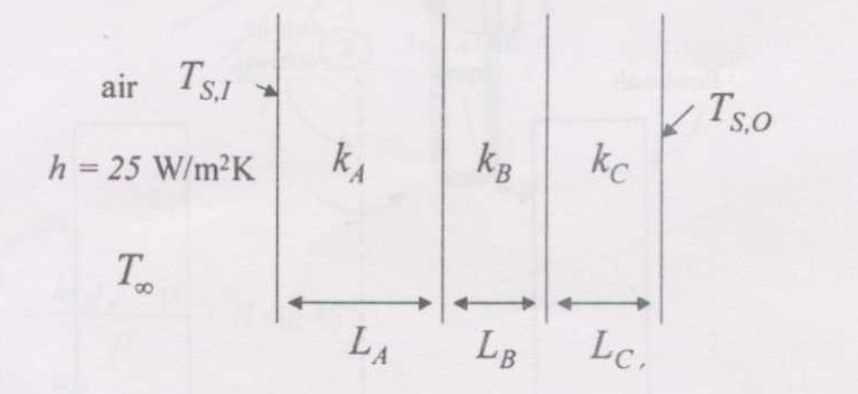
\includegraphics[width=0.5\linewidth]{GATE-PI-2020/42.png} 
    \caption{}
    \label{42}
\end{figure}
\vspace{1cm}

% Q.43
\item To manufacture a product by casting, molten metal is poured in a cavity of rectangular cross section in a sand mold with a side blind riser as shown in the figure. The dimensions of the mold cavity are $60~\text{cm} \times 40~\text{cm} \times 20~\text{cm}$.

\begin{figure}[H]
    \centering
    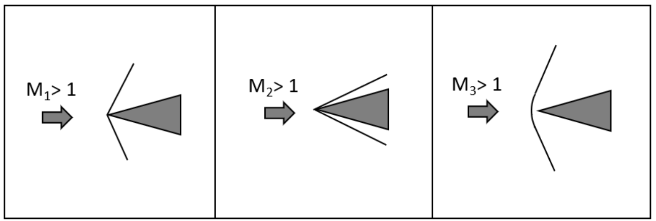
\includegraphics[width=0.5\linewidth]{GATE-PI-2020/43.png}
    \caption{}
    \label{fig:moldriser}
\end{figure}

The riser is cylindrical in shape with diameter equal to height. It is required that the solidification time of the riser should be 25\% greater than that of the mold. Using Chvorinova's rule, the diameter of the riser (rounded off to one decimal place) in cm should be \underline{\hspace{2cm}}.
\vspace{1cm}
\newpage
% Q.44
\item A cylindrical billet of 90 mm diameter is extruded to produce an I-section as shown in the figure (all dimensions in mm).

\begin{figure}[H]
    \centering
    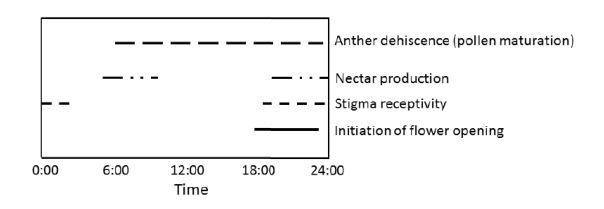
\includegraphics[width=0.5\linewidth]{GATE-PI-2020/44.png} 
    \caption{}
    \label{fig:extrudesection}
\end{figure}

The total extrusion pressure ($p_e$) in MPa required for the above process is given by
\[
p_e = \sigma_m \left[ 0.8 + 1.2 \ln\left( \frac{A_0}{A_f} \right) \right]
\]
where, $\sigma_m$ is the mean flow stress of the material, and $A_0$ and $A_f$ are the initial and the final cross-sectional areas, respectively. If the mean flow stress of the extruded material is 80~MPa, the force required for the above extrusion (rounded off to one decimal place) in kN is \underline{\hspace{2cm}}.
\vspace{1cm}

% Q.45
\item The heat generated in a resistance spot welding operation for joining two metal sheets with a certain set of process parameters is 2000~J. For a second spot welding operation on the same sheets without any change in the overall resistance of the system, the current is increased by 25\% and the time for which the current is applied is reduced to half. The heat generated in the second operation (rounded off to one decimal place) in J is \underline{\hspace{2cm}}.
\vspace{1cm}

% Q.46
\item A vertical boring operation is performed in a cast iron plate to enlarge a blind hole to a diameter of 25~mm up to a depth of 100~mm in a single pass. The cutting speed and the feed used in the process are 100~m/min and 0.1~mm/rev, respectively. Considering the allowance for tool approach as 2~mm, the actual machining time (rounded off to two decimal places) in minutes is \underline{\hspace{2cm}}.
\vspace{1cm}

% Q.47
\item For a particular tool-workpiece combination, the value of exponent $n$ in Taylor's tool life equation is $0.5$. If the cutting speed is reduced by $50\%$ keeping all the other machining conditions same, the increase in tool life in \% is \underline{\hspace{2cm}}.
\vspace{1cm}

% Q.48
\item In a waterjet machining process, the water pressure used is 500~MPa. The diameter of orifice of the nozzle through which the waterjet comes out is 0.25~mm. Neglecting frictional and other losses, and using the density of water as 1000~kg/m$^3$, the mass flow rate of the waterjet (rounded off to two decimal places) in kg/min is \underline{\hspace{2cm}}.
\vspace{1cm}

% Q.49
\item The movement along the $z$-axis of a CNC drilling machine is controlled by using a servo motor, a lead screw and an incremental encoder. The lead screw has 2 threads/cm and it is directly coupled to the servo motor. The incremental encoder attached to the lead screw emits 100 pulses/revolution. The control resolution in microns is \underline{\hspace{2cm}}.
\vspace{1cm}

% Q.50
\item A project consists of seven activities as listed in the table. The time required for each activity and its immediate predecessor(s) are also given.

\begin{center}
\begin{tabular}{|c|c|c|}
\hline
Activity & Time required & Immediate \\
         & (in weeks)    & Predecessor(s) \\
\hline
P & 7 & - \\
Q & 4 & - \\
R & 2 & Q \\
S & 11 & P \\
T & 9 & P, R \\
U & 9 & Q \\
V & 4 & T, U \\
\hline
\end{tabular}
\end{center}

The project completion time using Critical Path Method (CPM) in weeks is \underline{\hspace{2cm}}.
\vspace{1cm}
% Q.51
\item A company is planning to procure a machine to produce a component. There are two alternatives available - machine A and machine B. The cost of producing $x$ units of the component (in Rs.) using machine A is given as $C_A(x) = 10000 + 170x + x^2$. The cost of producing $x$ units of the component (in Rs.) using machine B is given as $C_B(x) = 15000 + 400x$. If machine B is to be preferred, then the minimum number of units to be produced should be \underline{\hspace{2cm}}.

\vspace{1cm}

% Q.52
\item The availability of an old photocopier was $90\%$ and the Mean Time Between Failure (MTBF) was $200$ days. It has been replaced with a new photocopier having an availability of $95\%$. Now, the Mean Time to Repair (the time during which the photocopier is unavailable for service) has increased by $5$ days. The MTBF of the new photocopier (rounded off to the nearest integer) in days is \underline{\hspace{2cm}}.

\vspace{1cm}

% Q.53
\item A car company manufactures 200 units of a component per day. The component is installed in different car models at a rate of 15,000 units per year. The company operates its production facility 300 days per year to manufacture the component. The setup cost for each production run is Rs. 200 and the inventory holding cost per year is Rs. 2 per unit. The Economic Production Quantity (EPQ) is \underline{\hspace{2cm}}.

\vspace{1cm}
\newpage
% Q.54
\item A company has to perform five tasks (P, Q, R, S and T) to make an assembly. Task times and immediate predecessors of the tasks are listed below. If an assembly line is designed to obtain the maximum output rate, the efficiency of the line in \% is \underline{\hspace{2cm}}.

\begin{center}
\begin{tabular}{|c|c|c|}
\hline
Task & Task time (Seconds) & Immediate predecessor(s) \\
\hline
P & 20 & -- \\
Q & 25 & P \\
R & 10 & Q \\
S & 15 & Q \\
T & 25 & R, S \\
\hline
\end{tabular}
\end{center}

\vspace{1cm}

% Q.55
\item In a work study experiment, it is observed that a worker completes a job in an average time of 15 minutes with a performance rating of 120\%. The time required for another worker having a performance rating of $80\%$ to complete the same job (rounded off to one decimal place) in minutes is \underline{\hspace{2cm}}.

\vspace{5cm}
\textbf{\Large END OF GATE PAPER PI}











   
\end{enumerate}



\end{document}